% 第4章
\section{システム設計(\textcolor{orange}{61\%})}
  \label{sec:システム設計}
    \par
  
  \subsection{システム要件の定義(\textcolor{green}{100\%})}
    \label{sec:システム要件の定義}
      \par システム要件は,本研究で構築するシステムの目的や機能,性能などの満たすべき要件を指す.システムの利用者のニーズやシナリオ等を定義するユーザ要件,システムの機能面における必要動作を定義する機能要件,システムの機能以外の面におけるシステムの振る舞いを定義する非機能要件に大別してまとめる.また,特に断りが無い限り,APIとしてのシステム要件としての定義をまとめる.ただし,自転車割り当て機能に関しては数理最適化処理などの計算量が多くなる処理を行う必要があるためこの限りではない.

      \subsubsection{ユーザ要件(\textcolor{green}{100\%})}
        \label{sec:ユーザ要件}
          \par ユーザ要件はシステム設計の出発点であり,ユーザのニーズを正確に把握することはサービスを提供する上で非常に重要な要素となる.本システムにて考慮する必要のあるユーザグループやそのペルソナ,ユーザシナリオについてまとめる.
          \par 本システムにおける主なユーザグループとしては3つに分類することができる.シェアサイクルの貸し手ユーザとなる自転車オーナと,シェアサイクルの借り手ユーザとなる自転車利用者,システム管理者である.自転車オーナは,自身が所有する自転車を,自身が利用しない時間帯にシェアリングの対象として第三者が利用可能な状態にして貸し出す.自転車利用者は,利用時の位置情報や目的地情報に基づき,目的地で乗り捨て可能な,個人の自転車オーナが所有している自転車を利用して移動する.システム管理者は,それぞれの地域で本システムをデプロイしてサービス運営を行う.必要に応じて,乗り捨てられた自転車をその自転車オーナの元に戻す「再配置作業」もシステム管理者が実施することとなる.
          \par それらのユーザグループを元に,各ユーザーグループの代表的なペルソナを定義する.まずは自転車利用者のペルソナについて定義する.自転車利用者は,手軽に自転車を借りたい地方在住の通勤者や観光客であるとする.公共交通機関を利用する程でも無い距離感の移動において,より効率的に移動するための手段として自転車を利用したいが,自身は自転車を保有しておらず,都市部と比較してシェアサイクルポートが点在しているわけでもないため,移動の効率化に課題を感じている.次に,自転車オーナのペルソナについて定義する.自転車オーナは,1台以上の自転車を保有している一方で頻繁にその自転車を利用しているわけではない人物とする.自分の労力を極力費やすことなく,自転車をシェアし,リソースを有効活用できればそれに越したことはないと感じている.システム管理者のペルソナは明確に定義しないが,各地域でシェアサイクル事業を展開したい個人もしくは行政とする.
          \par 定義したペルソナから,具体的なユーザシナリオを策定する.まず自転車オーナが,自身の利用していない自転車または,利用している自転車の利用していない時間帯を登録し,自転車利用者が利用可能な自転車がどの自転車であるかを明確にする.続いて,自転車ユーザが自転車の利用リクエストを送信し,本システム内のアルゴリズムによって割り当てられた自転車を利用する.自転車ユーザは自身の目的地付近にて自転車の乗り捨てを許容する.他の自転車ユーザからのリクエストによって自転車がそのオーナの元に帰ってくる,もしくは,システム管理者によって再配置するシナリオによって乗り捨て可能とする.
          
          
      \begin{table}[htbp]
        \caption{機能毎の機能要件一覧}
        \label{tab:機能毎の機能要件一覧}
        \centering
        \begin{tabular}{|l|p{4cm}|} \hline
          機能名 & 概要 \\ \hline
          ユーザ登録・認証 & ユーザがシステムに登録し,認証を行う機能 \\ \hline
          自転車登録 & 自転車オーナが自転車を登録する機能 \\ \hline
          自転車リクエスト & 自転車ユーザが自転車を利用するリクエストを行う機能 \\ \hline
          自転車割り当て & ユーザからのリクエストに対して最適な自転車を割り当てる機能 \\ \hline
          自転車利用確定 & 割り当てられた自転車に対して利用確定する機能 \\ \hline
          スマートロック操作 & 自転車ユーザがスマートロックを操作する機能 \\ \hline
          支払い処理 & 自転車ユーザが利用料金を支払う機能 \\ \hline
          評価・レビュー & ユーザが評価やレビューを投稿・閲覧する機能 \\ \hline
        \end{tabular}
      \end{table}


      \subsubsection{機能要件(\textcolor{green}{100\%})}
        \label{sec:機能要件}
          \par IEEE 830\scalebox{0.7}{\cite{392555}}によると,機能要件とは,ソフトウェアが入力を受け入れて処理し,出力を処理および生成する際に行うべき基本的な動作を定義するものであり,ソフトウェア要件仕様の中でも特に重要な部分であると述べられている.本システムにおいて定義すべき機能要件についてまとめる.
          \par 機能要件を機能ごとに整理・分類し,システムの全機能を一覧にした表を表\ref{tab:機能毎の機能要件一覧}に示す.各機能について詳細を定義する.
          \par ユーザ登録・認証機能は,ユーザがシステムを利用するためのアカウント作成と認証を提供することを目的とする.詳細な機能として,新規ユーザ登録やログイン・ログアウト機能,パスワードリセット・変更機能を含める.必要に応じてソーシャルメディア連携による登録やログインも含める選択肢も考えられる.メインとなるユーザ登録・認証機能については,ユーザ側の入力値に,ユーザ情報となる氏名やメールアドレス,パスワードを与える.入力値の結果としてユーザアカウントの作成確認や認証トークンの発行を行う.
          \par 自転車登録機能は,自転車オーナが自身の自転車をシステムに登録し,利用可能時間などの貸し出し条件を設定することを目的とする.種類やメーカ,写真や簡単な説明などの自転車情報や貸し出し可能日時,自転車の位置情報などの登録を可能とする.ログインしているユーザに自転車オーナステータスが存在することを前提とし,自転車の詳細情報や貸し出し条件を入力値として渡す.出力結果として登録完了確認メッセージや登録した自転車の一覧・編集画面を返す.
          \par 自転車リクエスト機能は,自転車ユーザがシェサイクルサービスを利用したい際に,システムにリクエストすることを目的とする.本システムにおいて,数理最適化ベースで割り当てを行うことを前提とした場合,一定期間のリクエストをストックする必要がある.本機能においてユーザリクエストをストックする機能も含める.リクエストする際に,自転車ユーザの現在地と目的地の位置情報を入力値として渡し,リクエストが完了した旨のメッセージを出力結果とする.
          \par 自転車割り当て機能は,複数のユーザからのリクエストを元に,ユーザビリティとシステム運用コストの観点から最適な自転車を割り当てることを目的とする.ユーザから最も近い位置に駐輪されている自転車を割り当てるモデルや数理最適化ベースで割り当てるモデル,機械学習ベースで割り当てるモデルなど用意し,複数の自転車割り当てモデルを選択することが可能であることも要件に含める.また,本機能は自転車リクエスト機能から呼び出される機能であり,クライアントから直接呼び出されることはない前提とする.割り当て処理に用いるモデルやユーザリクエスト,自転車ステータスを入力値として渡し,それらの情報から割り当てられた最適な自転車情報を出力する.
          \par 自転車利用確定機能は,自転車割り当て機能から出力された自転車に対して,その自転車を利用するか否かの最終判断を担うことを目的とする.自転車ユーザが割り当てられた自転車を利用することを確定した場合の自転車ステータスの更新処理は本機能の一部として含める.割り当てられた自転車の情報とそれを利用するか否かのブーリアン情報を入力として渡し,利用確定した自転車のスマートロック認証のためのトークン情報を出力結果として返す.
          \par スマートロック操作機能は,自転車に取り付けられたスマートロックに対して解錠・施錠を行うことを目的とする.自転車利用確定機能の出力から取得したスマートロック認証トークンと解錠・施錠を意味するバイナリ値を入力として渡し,実際のスマートロックの解錠・施錠動作が出力結果となる.
          \par 支払処理機能は,サービスの利用が完了したユーザから利用料を受け取り,自転車を貸し出したオーナへ貸し出し料を支払うことを目的とする.本機能においては支払機能コンポーネントとして提供されている外部サービスを利用して構築する.
          \par 評価・レビュー機能は,ユーザが評価やレビューを投稿・閲覧することで,個人間取引の中でも質の高い安定したサービス運営を実現させることを目的とする.ユーザのIDや評価数値,コメントなどを入力として渡し,評価完了後にはシステムのホーム画面へ遷移する.
      
      \subsubsection{非機能要件(\textcolor{green}{100\%})}
        \label{sec:非機能要件}
          \par 非機能要件とは,システムの機能以外の側面,すなわちシステムがどのように動作するかを規定する要件である\scalebox{0.7}{\cite{glinz2007non}}.\ref{sec:機能要件}項にて述べた機能要件が「システムは何をするか」を定義するのに対し,非機能要件では「システムはどのように振る舞うか」を定義する.ユーザ要件や機能要件と同様にシステム構築の重要な要素となり,主に,システムの品質や,信頼性,使いやすさ,保守性,セキュリティなどの面を保証する役割を果たす.
          \par 非機能要件として定義するカテゴリは,「性能」,「信頼性」,「可用性」,「セキュリティ」,「ユーザビリティ」,「保守性」,「拡張性」,「互換性」,「法的・倫理的要件」の通りに分類する.各カテゴリごとに具体的な非機能要件の定義内容についてまとめる.
          \par 性能要件では,システム全体におけるパフォーマンスの基準を定義する.数理最適化などの複雑な処理を行っている一方で,ユーザの待ち時間を最小限にして快適な操作性を実現する必要もあるため,ユーザがAPIに対してリクエストしてからレスポンスを返すまでの時間は500ミリ秒以内とする.また,サービスの利用拡大を見据え,ピーク時の負荷に耐え得るシステム性能を確保するため,一秒あたりの同時接続数500リクエストを処理可能とする.
          \par 信頼性要件では,稼働率やフォールトトレランスなどの,通常および異常な状況下でシステムがどの程度タスクを実行するべきかを定義する.稼働率に関しては,ユーザがいつでもサービスを利用できるようにするため,月間稼働率を99.9\%以上とする.また,フォールトトレランスに関しては,単一障害点を排除し,サービスの継続性を確保する目的で,障害発生時にもサービスを継続できる冗長構成を採用する.
          \par 可用性要件では,運用スケジュールなどのシステムを継続利用するための要件を定義する.特にメンテナンスウィンドウにおいて,ユーザの利用が少ない時間帯にメンテナンスを行い,可用性を高めることを目的として,計画メンテンナンスは深夜帯に限定し,ユーザへの影響を最小限にする.
          \par セキュリティ要件では,セキュリティに関する対策や目標,それに伴う機能を定義する.認証・認可に関しては,セキュリティレベルを高め,ユーザのアカウントを保護するため,ユーザ認証の際には多要素認証を導入し,不正アクセスを防止する.また,データ保護に関しては,データの盗聴や改ざんを防止し,プライバシーを保護するため,個人情報は暗号化して保存し,API通信にはSSL/TLSプロトコルを利用する.
          \par ユーザビリティ要件では,ユーザの使いやすさに対しての要件を定義する.UX(ユーザエクスペリエンス)を向上させ,サービスの利用促進につなげるため,特にAPI仕様書のUI(ユーザインターフェース)は直感的で分かりやすく設計する.また,多様なユーザが利用可能なインクルーシブなサービスを提供するため,多言語対応の観点から,API仕様書を日本語と英語で切り替え可能とする.さらに,ソースコードごとクローンし,ユーザがカスタマイズしたアプリケーションを構築する利用目的も考慮し,ローカル環境構築の手順をまとめたドキュメントも準備する.
          \par 保守性要件では,システムに異常が発生した場合の対応や障害監視システムやメンテナンスに関する要件を定義する.将来的な機能の追加やバグ修正を容易にするため,可読性の高いコードを作成し,マイクロサービスアーキテクチャに基づいた設計を行う.また,障害対応時にはそれに対応したログをドキュメントとして残す.データに関する保守について,データに異常が発生した場合はバックアップデータを利用して復元可能であり,取り扱われるデータはサービス提供期間中保持する.
          \par 拡張性要件では,将来的にシステムの性能をどのように拡張するするのかを定義する.サービスの成長に伴うアクセス増加に対応可能なスケーラブルなアーキテクチャであることを目指し,負荷の増大に応じでシステムリーソースを容易に拡張できるクラウドベースのアーキテクチャを採用する.
          \par 互換性要件では,異なるシステムが相互に適切に動作するために満たすべき条件や基準を定義する.特にAPI互換性について,外部サービスやアプリケーションとの連携を継続的に可能とするため,APIはバージョン管理を行い,後方互換性を維持する.
          \par 法的・倫理的要件では,法的及び倫理的観点からシステムがどのように振る舞うべきかを定義する.法令順守とユーザの信頼確保のため,個人情報保護法に準拠し,適切なデータ管理を行う.一方で,未だ実社会に存在しない「個人間の自転車共有」の実現を試みていることから,自転車の乗り捨て問題が課題として挙げられるが,本研究としては簡単のため自転車の乗り捨てに係る法的問題は考慮しないこととする.
          \par ここでまとめた非機能要件に関しては,実装時にその優先度を設定し,優先度に沿って実装する.なお,その際にそれぞれの要件が現実的で達成可能化の妥当性を確認し,必要に応じて調整する.
      
  \subsection{全体アーキテクチャの設計(\textcolor{green}{100\%})}
    \label{sec:全体アーキテクチャの設計}
      \par 改めて,本研究を通して最終的に目指していることは,個人間(C2C)ドックレスシェアサイクルシステムを実現させることである.それを実現する上で重要なファクターが3つ存在すると考えている.1つ目は,オーナに対して,自身の自転車に取り付けてもらうためのIoT及びスマートロックである.2つ目は,オーナとユーザのインターフェースとなるアプリケーションである.そして3つ目は,個人間の自転車シェアリングで尚且つ乗り捨て可能なシステムを実現するためアルゴリズムである.
      \par 3つ目に述べたファクターであるアルゴリズムについては\ref{sec:マッチングモデルの設計}にて後述する.そのため,本章においては,1つ目と2つ目に挙げたスマートロックとアプリケーションについての包括的なアーキテクチャを設計することを目的とする.

      \subsubsection{システム構成図(\textcolor{green}{100\%})}
        \label{sec:システム構成図}
          \par システム構成図は,定義した要件に対して,システムの各部分においてどのように反映させるかを視覚的に示す役割を果たす.本研究において構築するシステム構成の全体像としては,既存のシェアサイクルサービスと比較した場合,図\ref{fig:本研究において構築するシステム構成の全体像}に示す通りとなる.既存のシェサイクルサービスでは事業者が提供しているシェアサイクルポートの設置位置に依存してサービスが展開される.一方で,本研究において構築するサービスモデルでは個人所有の自転車が駐輪されている駐輪場に依存してサービスを展開することが可能である.それ故に,個人所有の自転車で利用されているそれぞれの鍵の形態を考慮する必要性が課題として挙げられるが,ここではプロトタイプの提案として,後述する\ref{sec:スマートロックの構築}節及び\ref{sec:スマートロックの実装}節にて一般的な自転車に標準装備されているシリンダー式のリング錠を前提としたシステムを構成することとする.
           \par また,図\ref{fig:本研究において構築するシステム構成の全体像}に示したようなシステムを構成するにあたって,自転車の鍵をスマートロック化し,利用するユーザに応じてスマートロックを解錠する必要がある.そこで本研究では,スマートロックの認証において,NFCを用いたとデバイス認証と指紋を用いた生体認証の2つのパターンからそれぞれアプローチする.それぞれの認証についてのシステム構成の詳細は\ref{sec:スマートロックの構築}節及び\ref{sec:スマートロックの実装}節にて後述する.
           \par 本研究にて想定する具体的なシステムの利用順序は図\ref{fig:想定するシステム利用手順概要図}に示す通りである.構築したスマートロックを自転車のオーナが自身の自転車に取り付け,専用のモバイルアプリケーションにて,利用を希望しているユーザが利用しても良い時間帯を予め登録しておく.その後,ユーザは利用したい際にモバイルアプリケーションから利用したい時間帯とマッチする自転車を探し出し,利用の申請を行う.
           \par ただし,本研究においは,ここで説明しているモバイルアプリケーションの構築は対象外とし,スマートロックのプロトタイプ構築に限定している.
          
          \begin{figure}[htbp]
            \centering
            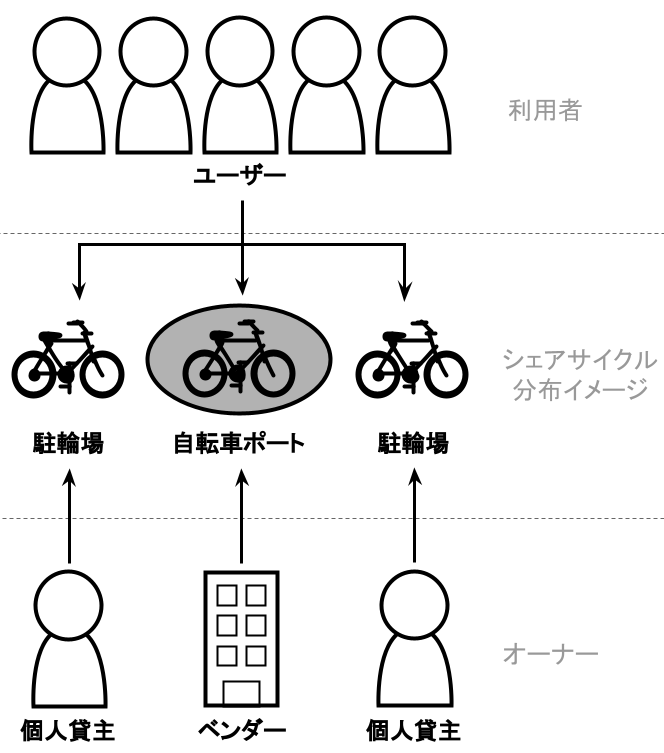
\includegraphics[scale=0.35]
            {figures/OverallImageOfSystemConfiguration.png}
            \caption{本研究において構築するシステム構成の全体像}
            \label{fig:本研究において構築するシステム構成の全体像}
          \end{figure}
          
          \begin{figure}[htbp]
            \centering
            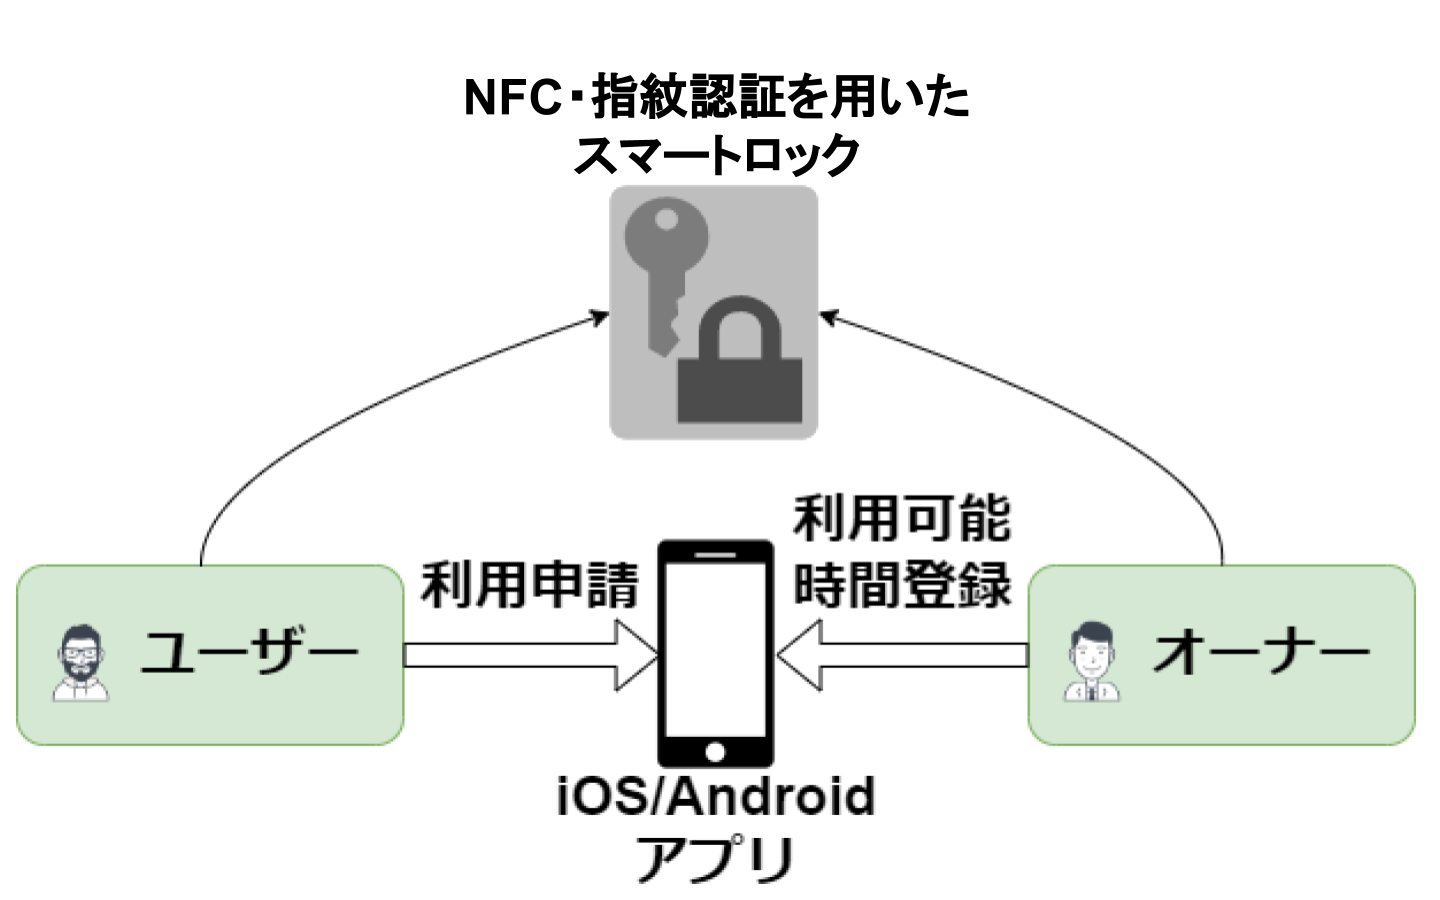
\includegraphics[scale=0.17]
            {figures/howToUse.png}
            \caption{想定するシステム利用手順概要図}
            \label{fig:想定するシステム利用手順概要図}
          \end{figure}
      
      \subsubsection{データフローの設計(\textcolor{green}{100\%})}
        \label{sec:データフローの設計}
          \par $\Box$ ER図・データの型についての話・データ保護についての話・データフロー設計において、システムのパフォーマンスを向上させるための工夫(キャッシュの利用、データの非同期処理、バッチ処理)・データ冗長性の排除(正規化、データの一元管理)
          \par データフロー設計とは,システムやアプリケーション内におけるデータの流れを視覚化し,設計するプロセスを意味する.データがどのように生成され,そのデータをどのように転送及び処理を行い,結果を格納し,さらに格納したデータをどのように使用するかを明確にするための重要な設計手法である.本研究にて構築するシステムで扱うデータの流れをデータフロー図を用いて簡潔にまとめる.なお,データフロー図には「レベル」の概念が存在し,レベルの数値が大きければ大きいほどデータフローが細分化され,システムの内のデータの流れがより具体的に表現される.一方で,レベルの数値が小さいければ小さいほどデータの流れが抽象的に表現される.
          \par レベル0のデータフロー図を図\ref{fig:レベル0のデータフロー図}の通りに表現する.レベル0では,システム全体の流れを最も抽象度高く簡略化して表現する.外部エンティティとして自転車を利用する自転車ユーザと自転車の提供者となる自転車オーナに限定し,自転車割り当てプロセスを介して自転車ユーザには割り当てられた自転車を,自転車オーナにはその結果を通知するフローを表している.
          \par レベル1のデータフロー図を図\ref{fig:レベル1のデータフロー図}の通りに表現する.レベル1では,より詳細に主要なプロセスやサブシステムを図示している.自転車ユーザからのリクエストは該当するデータベースへ一時的にストックされ,任意の時間幅でリクエストのバッチを取得する.自転車オーナは自転車登録プロセスを介して該当のデータベースへ自転車を登録し,リクエストバッチの取得プロセスの結果に基づいて自転車ユーザへ自転車を割り当てる.自転車ユーザが利用を確定した場合には,自転車データベースのレコードを更新し,スマートロック認証プロセスを介してユーザが自転車を利用できる権限を与える.同時に自転車オーナにも結果を通知する.
          \par ここで利用する主要なエンティティとしてユーザエンティティ,自転車エンティティ,ユーザリクエストエンティティが挙げられる.ただし,ここでのユーザエンティティについては,システムのユーザを指しており,自転車の利用者と自転車のオーナのどちらともをエンティティとして定義している.ユーザエンティティでは,ユーザに関する情報(ユーザID・氏名・メールアドレス・ユーザステータス・オーナステータス・住所など)を保持する.自転車エンティティでは,自転車に関する情報(自転車ID・所有者ID・車種名・ステータス・位置情報など)を保持する.ユーザリクエストエンティティでは,リクエストに関する情報(利用者ID・利用開始位置情報・目的地位置情報・利用開始時間・利用終了予想時間など)を保持する.
          \par 各プロセスにおけるデータの入力や取得は原則API通信を介して行う.入力データはクエリパラメータやエンドポイントのパスに含め,出力データはJSON形式で取得する.

          \begin{figure}[htbp]
            \centering
            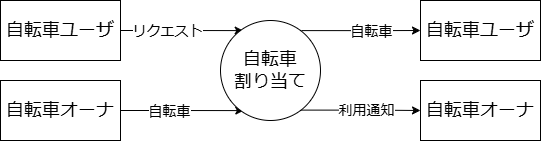
\includegraphics[scale=0.4]
            {figures/dfd-level0.drawio.png}
            \caption{レベル0のデータフロー図}
            \label{fig:レベル0のデータフロー図}
          \end{figure}

          \begin{figure*}[htbp]
            \centering
            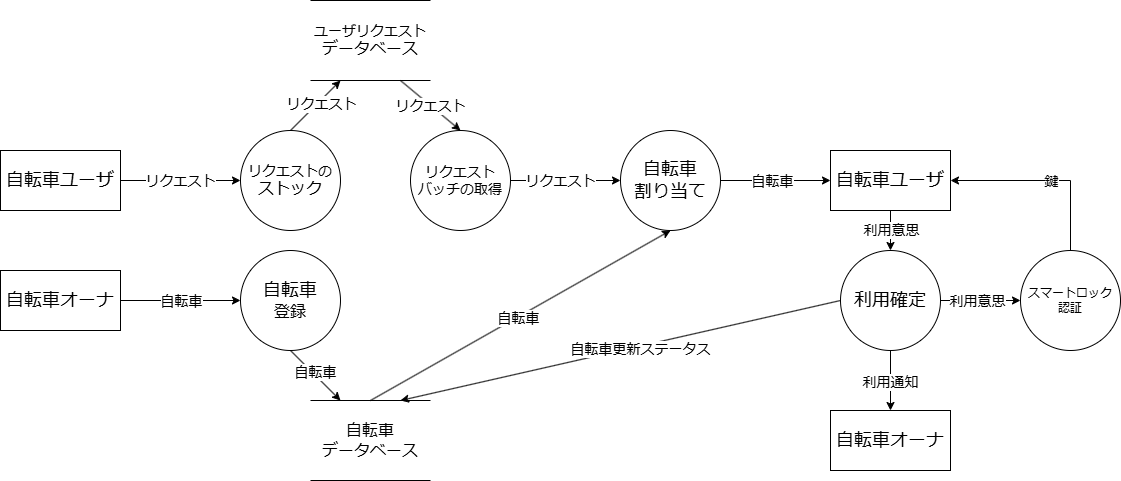
\includegraphics[scale=0.4]
            {figures/dfd-level1.drawio.png}
            \caption{レベル1のデータフロー図}
            \label{fig:レベル1のデータフロー図}
          \end{figure*}

  \subsection{スマートロックの構築(0\%)}
    \label{sec:スマートロックの構築}
      \par 
      
      \subsubsection{ハードウェア設計(0\%)}
        \label{sec:ハードウェア設計}
          \par ここでハードウェアについての要件定義(保守要件とか)を書く?
          
      \subsubsection{組み込みソフトウェアの開発(0\%)}
        \label{sec:組み込みソフトウェアの開発}
          \par
          
      \subsubsection{通信プロトコルの選定(0\%)}
        \label{sec:通信プロトコルの選定}
          \par
          
  \subsection{マッチングモデルの設計(0\%)}
    \label{sec:マッチングモデルの設計}
      \par

      \subsubsection{数理最適化モデルの定式化(\textcolor{green}{100\%})}
        \label{sec:数理最適化モデルの定式化}
          \par $\Box$ 変数や制約の数、計算複雑性について触れる。
          \par シェアサイクルサービスをCtoC化することによる特徴として,サービスを提供するために大量の自転車を予め確保する必要性がなく,個人が所有している未使用の自転車を有効活用することができる点や,都市部と地方で設置数に偏りが生じやすいポートに依存せず,ポートがない場所でも乗り捨てが可能となり,移動自由度の向上が期待できる点が挙げられる.また,自転車保有者側の観点においても,自転車を利用していない期間にそれをユーザに貸し出すことで,自身のリソースを有効活用できると捉えることもできる.一方で,ユーザに対して適切な自転車が割り当てられない場合や,既存のシェアサイクルシステムのようにユーザが好みの自転車を自由に選択することができる状況下においては,乗り捨てられた自転車とその保有者との位置関係が未知数となり,自転車を再配置する際に多くのコストを要することが想定される.
          
          \par そこで,個人所有の自転車を効率的にシェアし,乗り捨て可能なシェアサイクルシステムを実現するため,数理最適化ベースの自転車割り当てモデルを設計し,構築する.ユーザに自転車を割り当てるアルゴリズムを数式としてモデル化し,それに基づいて自転車割り当て処理が実行されるため,乗り捨て可能な個人所有自転車のシェアリングにおいて的確な割り当て結果を得ることが期待される.
          
          \par モデルの構築においては,整数計画法によるアルゴリズムを軸とする.
          
          \par 整数計画法は,一部または全ての決定変数が整数値のみをとるように制約された線形計画法である\scalebox{0.7}{\cite{wolsey2020integer}}.一方で,線形計画法では,変数は整数値以外も取ることができる.そのため,本研究でアプローチしているような整数計画問題を線形計画法を用いたプロセスで処理しようとすると,線形計画法による解が整数ではない場合,丸めた解が実行不可能または最適ではない可能性がある\scalebox{0.7}{\cite{hooker2024integer}}.整数計画法では,決定変数が整数であるべき多くの現実世界の状況をモデル化するのに役立つ\scalebox{0.7}{\cite{gomory1960integer}}.これらの観点を踏まえ,個人所有の自転車をユーザに割り当てる問題では,決定変数が「割り当てるか否か」のバイナリ変数であるべき問題であることより,整数計画法を用いたアルゴリズムを構築する.
          
          \par 前提条件として,本モデルが数理最適化ベースであることの利点を最大限活用するため,ユーザから自転車割り当てシステムに対するリクエストは1分間ストックし,ストックされたリクエストデータに対して毎分バッチ処理を実行する.また,シェアリングの対象は個人所有の自転車とし,ユーザ体験の観点において,移動自由度を向上させることを目的としてドックレスで乗り捨て可能なシステムを想定する.なお,乗り捨てによる自転車の不法駐輪等の法的な課題に関してはここでは考慮せず,あくまで自転車の割り当て問題として切り分けてモデリングする.
          
          \par 定式化で用いる集合やパラメータ,決定変数のそれぞれの記号と概説を表\ref{tab:記号の概説}に示す.ユーザリクエストの集合を$R$,シェアリングされる自転車の集合を$B$とする.ユーザ$r (r \in R)$に自転車$b (b \in B)$が割り当てられる前の初期状態として,ユーザとユーザがリクエストした時点での自転車の距離関係を表すパラメータを距離行列$d^{\text{init}}_{b,r}$とする.ユーザ$r (r \in R)$に自転車$b (b \in B)$が割り当てられ,ユーザが割り当てられた自転車に乗って移動したと仮定した場合のその後の自転車の位置と自転車の所有者までの距離関係を表すパラメータを距離行列$d_{b,r}$とする.
          
          \begin{table}[htbp]
            \caption{記号の概説}
            \label{tab:記号の概説}
            \centering
            \begin{tabular}{c p{6cm}}
              \hline 
              記号 & 説明 \\
              \hline
              $R$ & ユーザリクエストの集合 \\
              $B$ & シェアリングされる自転車の集合 \\
              $d^{\text{init}}_{b,r}$ & ユーザ $r(r \in R)$ と自転車 $b(b \in B)$ の割り当て前の距離行列\\
              $d_{b,r}$ & ユーザ $r (r \in R)$ に自転車 $b (b \in B)$ が割り当てられて移動した後の距離行列 \\
              $x_{b,r}$ & ユーザ $r (r \in R)$ に自転車 $b (b \in B)$ が割り当てられたか否かの二値変数行列 \\
              \hline
            \end{tabular}
          \end{table}
          
          \par 決定変数については,ユーザ$r (r \in R)$に自転車$b (b \in B)$が割り当てられたか否かの二値変数行列$x_{b,r}$とする.ユーザ$r$が自転車$b$を利用する場合に1,そうでなければ0のバイナリ値を持つ.
          
          \par 目的関数は\ref{equ:目的関数}式の通りに定義する.
          
          \begin{equation}\label{equ:目的関数}
            \min \left( \sum_{b \in B}\sum_{r \in R}d_{b,r}x_{b,r} - \alpha\sum_{b \in B}\sum_{r \in R}x_{b,r} \right)
          \end{equation}
          
          \begin{equation}\label{equ:移動後の距離最小化}
            \min \left( \sum_{b \in B}\sum_{r \in R}d_{b,r}x_{b,r} \right)
          \end{equation}
          
          \begin{equation}\label{equ:割り当て成功率最大化}
            \max \left(\sum_{b \in B}\sum_{r \in R}x_{b,r} \right)
          \end{equation}
          
          \par 第1項の部分については,\ref{equ:移動後の距離最小化}式に示す通り,ユーザが割り当てられた自転車に乗って移動した後の自転車とその自転車の所有者までの距離を最小化する.例えば,あるユーザからのリクエストがあった場合,そのユーザの現在地と目的地,リクエストされた時点での自転車とその自転車の所有者までの位置関係が図\ref{fig:ユーザと自転車の初期位置とリクエスト方向}の状態であったとする.なお,自転車の位置は自転車のアイコンで,自転車の所有者の位置は家のアイコンで表し,所有関係は色に対応している.この場合,\ref{equ:移動後の距離最小化}式に従うと,ユーザには緑色の自転車が割り当てられる.ユーザが移動した直後の状態が図\ref{fig:自転車割り当て・移動後の位置関係}に示す通りとなり,橙色の自転車が割り当てられた場合と比較して,点線で示した自転車とその自転車の所有者との距離の総和が小さくなる.
          
          \begin{figure}[htbp]
            \centering
            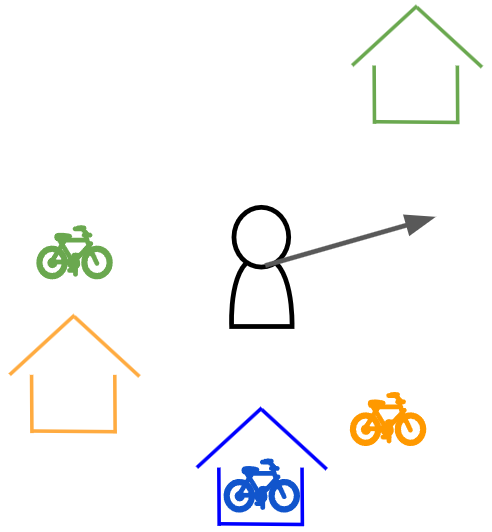
\includegraphics[scale=0.6]
            {figures/subjectFunction1-0.png}
            \caption{ユーザと自転車の初期位置とリクエスト方向}
            \label{fig:ユーザと自転車の初期位置とリクエスト方向}
          \end{figure}
          \begin{figure}[htbp]
            \centering
            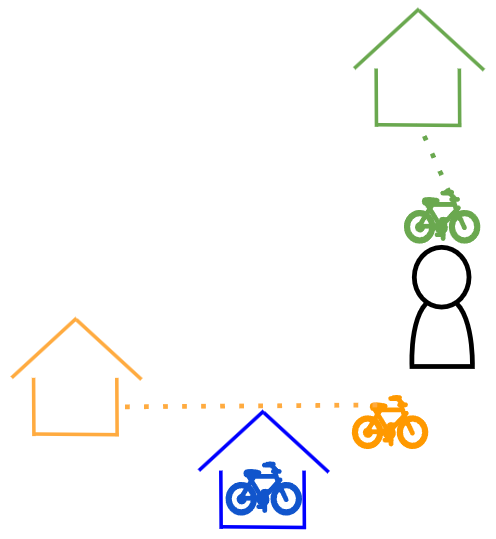
\includegraphics[scale=0.6]
            {figures/subjectFunction1-1.png}
            \caption{自転車割り当て・移動後の位置関係}
            \label{fig:自転車割り当て・移動後の位置関係}
          \end{figure}
          
          \par 第2項の部分については,\ref{equ:割り当て成功率最大化}式に示す通り,可能な限り多くのユーザに自転車を割り当てる最大化を行う.\ref{equ:移動後の距離最小化}式のみを目的関数として定義した場合,全ての自転車が所有者の手元にあるような極端な状況ではユーザに自転車を一切割り当てない選択をすることが,割り当て移動後の自転車とその自転車の所有者までの距離が最小化される結果となり,最適と判断されてしまう.サービスとしてもユーザに自転車が割り当てられることで初めて機能するため,\ref{equ:割り当て成功率最大化}式を目的関数の一部としている.
          
          \par なお,\ref{equ:移動後の距離最小化}式と\ref{equ:割り当て成功率最大化}式は最小化と最大化のトレードオフの関係にあるため,\ref{equ:割り当て成功率最大化}式に対してトレードオフの調整を行う重み$\alpha$を掛け合わせ,このトレードオフの最適値を探る.ただし,$\alpha$は非負であることを保証し,指定が無い場合は$\alpha=1$とする.\ref{equ:割り当て成功率最大化}式に対して$-\alpha$を掛け合わせることで,目的関数全体として最小化を行う.
          
          \par 制約条件は\ref{equ:半径制約}式から\ref{equ:人対自転車}式の通りに定義する.
          
          \begin{equation}\label{equ:半径制約}
            x_{b, r} \leq \mathbb{I}(d^{\text{init}}_{b, r} \leq 250), \forall b \in B, \, \forall r \in R
          \end{equation}
          
          \begin{equation}\label{equ:自転車対人}
            \sum_{r \in R}x_{b,r} \leq 1, \forall b \in B
          \end{equation}
          
          \begin{equation}\label{equ:人対自転車}
            \sum_{b \in B}x_{b,r} \leq 1, \forall r \in R
          \end{equation}
          
          \par \ref{equ:半径制約}式は,ユーザから半径250m以内の自転車のみを割り当てる制約を意味する.図\ref{equ:半径制約}に示すように,ユーザから半径250mの範囲外に位置する自転車は割り当ての対象外となる.\ref{equ:自転車対人}式は,図\ref{fig:自転車に割り当てられるユーザは1人以下}に示すように,自転車に割り当てられるユーザは1人以下であることを定義し,\ref{equ:人対自転車}式は,図\ref{fig:ユーザに割り当てられる自転車は1台以下}に示すように,ユーザに割り当てられる自転車は1台以下であることを定義する.これらの制約条件を設けることによって,ユーザから遠く離れた場所に位置する自転車の割り当てや,利用する自転車がユーザ同士で重複して割り当てられること,ユーザが複数台の自転車を利用して移動することを防ぐ.
          
          \begin{figure}[htbp]
            \centering
            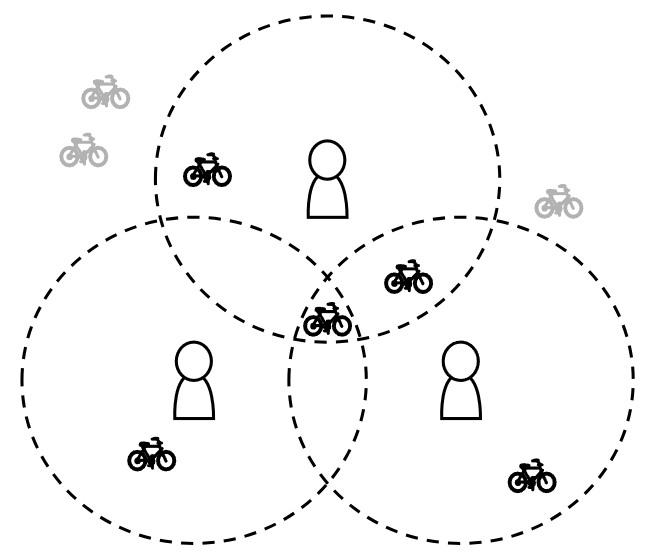
\includegraphics[scale=0.45]
            {figures/objectFunction1.png}
            \caption{割り当て許容距離に含まれている自転車の状態}
            \label{fig:割り当て許容距離に含まれている自転車の状態}
          \end{figure}
          
          \begin{figure}[htbp]
            \centering
            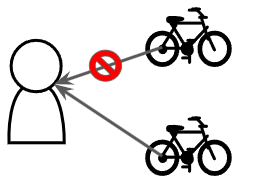
\includegraphics[scale=1.2]
            {figures/objectFunction2.png}
            \caption{自転車に割り当てられるユーザは1人以下}
            \label{fig:自転車に割り当てられるユーザは1人以下}
          \end{figure}
          
          \begin{figure}[htbp]
            \centering
            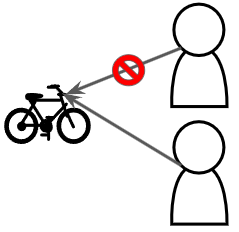
\includegraphics[scale=1.2]
            {figures/objectFunction3.png}
            \caption{ユーザに割り当てられる自転車は1台以下}
            \label{fig:ユーザに割り当てられる自転車は1台以下}
          \end{figure}

      \subsubsection{機械学習モデルの設計(0\%)}
        \label{sec:machine_learning_model_design}
          \par

  \subsection{APIの設計方針(0\%)}
    \label{sec:api_design_policy}
      \par
      
      \subsubsection{API機能要件の定義と設計(\textcolor{green}{100\%})}
        \label{sec:definition_of_api_function}
          \par API(Application Programming Interface)はアプリケーションとプログラミング的なやり取りを可能とするインターフェイスである.標準プロトコルを用いて文書化され,クライアントとサーバーの両方がそのAPIドキュメントに従っている限り,通信は期待通りに実行される.詳細は\ref{sec:コア技術の活用}節にて論じた.本研究において構築する自転車割り当てモデルをアプリケーション上のサービスとしてユーザに価値提供するためにAPIを利用する.
          \par APIの設計においてはREST APIの設計原則に準拠して設計する.特に,RESTの設計原則ではステートレスなアーキテクチャであることが挙げられており,これによってスケーラビリティや信頼性の向上が期待できる.需要を予測することが難しいCtoCシェアサイクルサービスにおいて,ニーズに合わせたサーバー処理が求められることから適切であると判断した.また,自転車のスマートロックなどのIoTデバイスとの連携においても,軽量であり様々なIoTデバイスとの通信に広く利用されている点も選定基準の1つである.
          \par \ref{sec:システム要件の定義}節にて定義したシステム要件から導出される,APIが提供するべき具体的な機能として,マイクロサービス単位で換算すると5つである.自転車割り当てサービス・自転車利用サービス・ユーザ管理サービス・自転車管理サービス・スマートロック操作サービスである.なお,マイクロサービスとは,マイクロサービス分野をリードする著者の1人であるSam Newman氏によると「一体となって動作する,小規模な自律的なサービス」と定義されている\scalebox{0.7}{\cite{newman2021BuildingMicroservices}}.また,James Lewis氏とMartin Fowler氏の記事によると,「1つのアプリケーションを一連の小さなサービスの組み合わせとして開発するアプローチ.これらのサービスはそれぞれの独自のプロセスで実行され,軽量なメカニズム(多くの場合はHTTPリソースAPI)を用いて通信する」と定義されている\scalebox{0.7}{\cite{Microservices}}.これらより,システムの各コンポーネントを個別にデプロイ可能なサービスとしてカウントできる単位をマイクロサービスとして定義する.
          \par 上記のサービスに基づき,必要なAPI機能となるエンドポイントを表\ref{tab:Bikeying API エンドポイント一覧}に一覧化する.なお,本研究にて構築するAPIをBikeying APIと命名し,以後その名称を用いる.自転車割り当てサービスでは,本研究で構築する自転車割り当てモデルのメイン処理を実装し,ユーザのリクエストに基づいた最適な自転車を割り当て,レスポンスする.自転車利用サービスは,実際にユーザが自転車を検索し,予約する際に,クライアントと自転車割り当てサービスとのインターフェイスとしての役割を果たす.ユーザのリクエストをある一定期間ストックする場合などに効果を発揮する.自転車管理サービス及びユーザ管理サービスでは,それぞれ自転車やユーザの追加や削除,ステータスの管理を行う責務を果たす.スマートロック操作サービスでは,自転車割り当てサービスや自転車利用サービスの結果に基づき,対象のスマートロックの解錠・施錠をAPI経由で制御できるようにする.
          \par ここで定義したBikeying APIのそれぞれのマイクロサービス間の基本的な関連性と,クライアントやIoTスマートロックとのインターフェースとしての立ち位置の概要を図\ref{fig:サービス間とインターフェースの関連}に示す.自転車利用サービスを軸として,クライアントからのリクエストを各々の責務を果たすマイクロサービスへと分散し,レスポンスする.IoTスマートロックの操作が必要となる場合は,図\ref{fig:サービス間とインターフェースの関連}に示す通り,スマートロック操作サービスがそのインターフェースとしての役割を果たす.

          \begin{table*}[t]
            \caption{Bikeying API エンドポイント一覧}
            \label{tab:Bikeying API エンドポイント一覧}
            \centering
            \begin{tabular}{|p{3.5cm}|l|p{5cm}|l|l|} \hline
              マイクロサービス & エンドポイント & 説明 & HTTPメソッド & 認証 \\ \hline
              自転車管理サービス & \url{/bikes} & 自転車の現在の利用ステータスを取得する & GET & 必須 \\ \cline{2-5}
              & \url{/bikes} & 自転車の現在の利用ステータスを更新する & PUT & 必須 \\ \cline{2-5}
              & \url{/bikes} & シェアリング可能な自転車を追加する & POST & 必須 \\ \cline{2-5}
              & \url{/bikes} & 自転車をシェアリングの対象から削除する & DELETE & 必須 \\ \hline
              自転車割り当てサービス & \url{/bikes/dispatch} & ストックされたリクエストから最適な自転車を割り当てる & GET & 必須 \\ \hline
              自転車利用サービス & \url{/bikes/requests} & ユーザの現在地座標などの条件に基づいたリクエストをストックする & POST & 必須 \\ \cline{2-5}
              & \url{/bikes/reserve} & 特定の自転車の利用を確定・予約する & POST & 必須 \\ \hline
              ユーザ管理サービス & \url{/users/signup} & 新規ユーザ登録 & POST & なし \\ \cline{2-5}
              & \url{/users/login} & ユーザのログイン処理 & POST & なし \\ \cline{2-5}
              & \url{/users/logout} & ユーザのログアウト処理 & POST & 必須 \\ \cline{2-5}
              & \url{/users/{userId}} & ユーザのプロフィール情報を取得する & GET & 必須 \\ \cline{2-5}
              & \url{/users/{userId}} & ユーザのプロフィール情報を更新する & PUT & 必須 \\ \hline
              スマートロック操作サービス & \url{/{lockId}/unlock} & 指定されたスマートロックを解錠する & POST & 必須 \\ \cline{2-5}
              & \url{/{lockId}/lock} & 指定されたスマートロックを施錠する & POST & 必須 \\ \cline{2-5}
              & \url{/{lockId}/status} & スマートロックの状態を取得する & GET & 必須 \\ \hline
            \end{tabular}
          \end{table*}

          \begin{figure}[htbp]
            \centering
            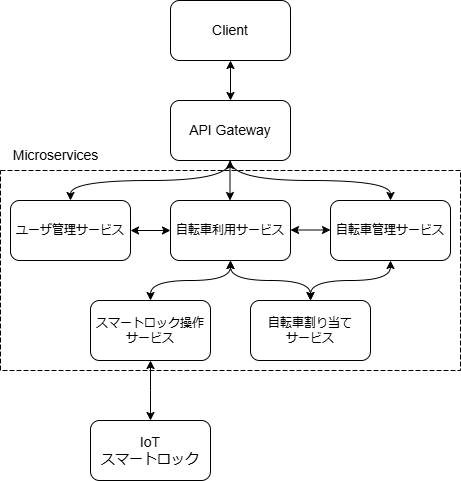
\includegraphics[scale=0.5]
            {figures/microservice-architecture.png}
            \caption{サービス間とインターフェースの関連}
            \label{fig:サービス間とインターフェースの関連}
          \end{figure}

      \subsubsection{セキュリティと認証の設計(\textcolor{green}{100\%})}
        \label{sec:security_and_authentication_design}
          \par $\Box$ 認証シーケンス図作成したい
          \par APIのセキュリティを考える上で認証及び認可の設計は,システムの信頼性とデータ保護を確保するために非常に重要であり,避けて通ることはできない.不適切なセキュリティ設計は,データの漏洩や不正アクセスなどの深刻な問題を引き起こす可能性がある.実際にAPI認証システムの脆弱性による被害が発生してる事例が存在する.例として,本研究と似通ったライドシェアサービスを展開しているUber社の事例を紹介する.2016年に,Uber社の開発者用APIキーがGitHubに公開されたことをきっかけに,Uber社が利用してる第三者機関のクラウドベースのサーバーにてユーザデータに不正なアクセスがあったことが発覚しした.APIキーを利用した攻撃により,日本でもおよそ10万人の乗客及びドライバに関する情報が漏洩したとされている\scalebox{0.7}{\cite{uber2016dataincident}}.そのため,本項では堅牢なシステム構築の重要な要素となるAPIにおける認証および認可を設計する.
          \par 認証とはAPIを利用しようとしてるユーザやアプリケーションが「誰であるか」を確認するプロセスである.これは「本人確認」に相当し,ユーザがAPIにアクセスするために提供したAPIキーやトークンなどが正しいかを判定する.一方で,認可とは認証済みのユーザやアプリケーションが「何をすることを許可されているか」を制御するプロセスである.これは「権限管理」に相当し,認証後にそのユーザが特定のリソースや機能へのアクセスが許可されているかを判定する.
          \par APIの認証で用いられる重要なプロトコルとしてはOAuth(Open Authrization)やOpenID Connect,JWT(Json Web Token)の3つが挙げられる.
          \par OAuthは,OAuthプロバイダーを通して認証と認可を行う,アクセス委任の標準プロトコルである\scalebox{0.7}{\cite{oauth}}.一般に,アクセスはトークンの発行により許可され,そのトークンを用いることで外部サービスとの連携が容易である点が特徴である.
          \par OpenID Connectは,OAuthプロトコルをベースとして構築された認証プロトコルであり,このプロトコルを用いることで,クライアントは認可サーバーの認証結果に基づいてエンドユーザを検証することができる.また,同時にエンドユーザに必要なプロフィール情報などもRESTfulな形式で取得することが可能となる\scalebox{0.7}{\cite{openidconnectjapan}}.
          \par JWTは,認証や認可,セキュリティを容易に実装するために当事者間でデータを交換するための軽量な手段となるJSONドキュメントを表すトークンである\scalebox{0.7}{\cite{mahindraka2020insights}}.JWTはプライベートシークレットもしくは暗号鍵を用いて署名され,そのドキュメントにはトークンの発行者やその対象,有効期限などの情報を含んでいる.これはOAuthにおいてもOpenID Connectにおいてもユーザのアクセスの検証として用いられている.
          \par 本研究で構築するAPIの認証及び認可においては,マイクロサービスアーキテクチャを採用しており,サービス間での認証と認可に適している点と,簡易的な認証基盤を設計し構築に要する時間的コストを削減する点を鑑みてこれらの認証プロトコルを用いて構築する.
          \par そこで,JWTのペイロードのクレームに含まれているそれぞれの項目の設定値を定義する.JWTの発行者をしきべつするためのiss(issuer)にはBikeying APIのドメイン及びそのURLを定義する.サーバーにリクエストを送信するユーザを識別するためのsub(subject)には適当なuuidを定義する.JWTが意図する受信者を識別するためのaud(audience)にはローカルホスト環境で立ち上げるURLを定義する.JWTが発行された日時のタイムスタンプであるiat(issued at time)には現在時刻を定義する.JWTの有効期限を指定するexp(expiration time)には現在時刻から24時間後の時刻を定義し,このトークンの有効期限は24時間とする.認証プロトコルにはOpenID Connectを用いるため,scope(scope value)にその旨を定義する.実際に定義したpayloadはListing \ref{list:JWTペイロード}の通りである.
          \par APIサーバーに認可を追加するため,生成したJWTを利用してAuthミドルウェアを構築する.悪意のあるユーザに情報を与えないためにも,認証及び認可に失敗した場合は403レスポンスではなく404レスポンスを返すこととする.ただし,Swagger UIで構築しているAPI仕様書やOpenAPIのJSONエンドポイントに対して認可を設定すると全てのAPIのエンドユーザが利用できなくなる場合も想定されるため,この2点については認証及び認可の処理を通らないよう考慮する.
          \par さらにセキュリティの観点において,CORS(Cross-Origin Resource Sharing)ミドルウェアも追加する.CORSとは異なるドメインやプロトコル,ポートからリソースにアクセスすることを許可するメカニズムである.通常は異なるオリジンからのアクセスは制限されるが,指定されたHTTPヘッダーを使用することで制限を緩和し,異なるオリジンを跨いだリソースの共有を可能とする\scalebox{0.7}{\cite{dresen2020corsica}}.

\lstset{
  identifierstyle={\small},
  commentstyle={\smallitshape},
  keywordstyle={\small\bfseries},
  ndkeywordstyle={\small},
  stringstyle={\small\ttfamily},
  frame={tb},
  breaklines=true,
  columns=[l]{fullflexible},
  numberstyle={\scriptsize},
  stepnumber=1,
  lineskip=-0.5ex
}
\begin{lstlisting}[caption={JWTペイロード}, label={list:JWTペイロード}, basicstyle=\ttfamily\footnotesize]
payload = {
  "iss": "https://auth.bikeying.com",
  "sub": "12e49b07-5ff3-4e2d-bfdf-6ac315ce5f33",
  "aud": "http://127.0.0.1:8000/bikes",
  "iat": now.timestamp(),
  "exp": (now + timedelta(hours=24)).timestamp(),
  "scope": "openid",
}
\end{lstlisting}
